\documentclass{minesbeamer}
\usepackage{movie15}
\title{Theory and Methods for the Ferromagnetic Ising Model}
\subtitle{TTIC 31180}
\author[Jay Shen \and Mark Lee]{Jay Shen \and Mark Lee}
\date{5/21/2024} % or whatever the date you are presenting in is
% \copyrightnotice{Published by the American Institute of Aeronautics and Astronautics, Inc., with permission}

\begin{document}

\maketitle

\cutoc

\section{Review of the Ising Model}

\begin{frame}{What is an Ising Model?}
    \begin{columns}
        \begin{column}{0.6\textwidth}
            \begin{figure}
                \centering
                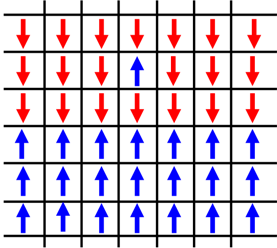
\includegraphics[height=0.7\textheight]{monte-carlo-ising-2.png}
            \end{figure}
        \end{column}
        \begin{column}{0.5\textwidth}
            \begin{itemize}
                \item The Ising model is used in statistical mechanics to describe ferromagnetism in materials.
                \item Each site on the lattice is associated with a spin, which represents the magnetic moment of an atom or molecule.
                \item The spins are subject to thermal fluctuations, causing them to flip between \{-1,1\}.
            \end{itemize}
        \end{column}
    \end{columns}
\end{frame}

\begin{frame}{Theory of the Ising Model}
    \begin{columns}
        \begin{column}{0.6\textwidth}
            \begin{itemize}
                \item A particle with magnetic moment $\overrightarrow{\mu}$ in an external magnetic field $\overrightarrow{B}$ has potential energy: $$U = -\overrightarrow{\mu}\cdot \overrightarrow{B}$$
                \item The magnetic moment also creates a magnetic field. The interaction between particles, denoted by exchange constants $J_{ij}$, also have potential energy: $$U = -J_{ij}\overrightarrow{\mu_1}\cdot\overrightarrow{\mu_2}$$
            \end{itemize}
        \end{column}
        \begin{column}{0.4\textwidth}
            \begin{figure}
                \centering
                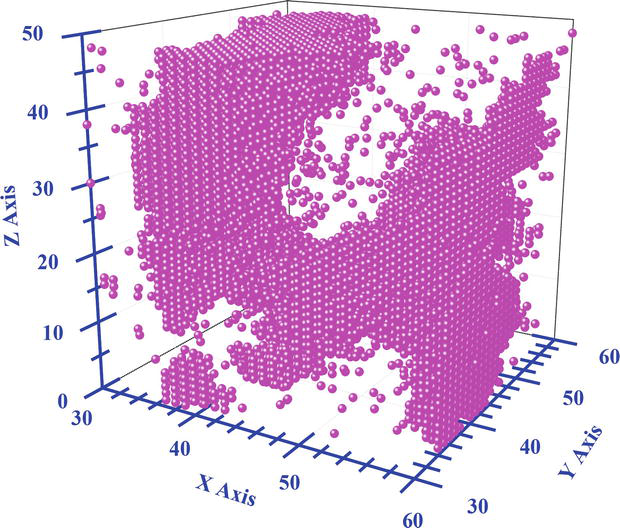
\includegraphics[height=0.6\textheight]{F5.png}
            \end{figure}
        \end{column}
    \end{columns}
\end{frame}

\begin{frame}{Theory of the Ising Model cont.}
    \centering
    \begin{itemize}
        \item So now we have a collection of particles in the presence of an external magnetic field. The Hamiltonian, which specifies the total energy of the system, is defined by the sum of all pairwise and all magnetic field energies:$$E = -\frac{1}{2}\sum_{i,j}J_{ij}\overrightarrow{\mu_i}\cdot\overrightarrow{\mu_j}-\sum_i \overrightarrow{\mu_i}\cdot\overrightarrow{B}$$
        \item This is intractable, and we can simplify it through several assumptions. By coalescing constants,$$E=-J\sum_i\sum_{j\in adj(i)}\sigma_i\sigma_j -\sum_i \sigma_i B_i$$
    \end{itemize}
\end{frame}

\begin{frame}{Theory of the Ising Model cont.}
    \centering
    \begin{itemize}
        \item Following the Boltzmann distribution, the probability of some state $\overrightarrow{\sigma}$ at inverse temperature $\beta$ is:$$P(\overrightarrow{\sigma}) = \frac{1}{Z}e^{-\beta E(\overrightarrow{\sigma})}$$
    \end{itemize}
\end{frame}

\section{Inference Using the Ising Model}

\begin{frame}{Make your presentation interactive}
    \begin{cublock}[What about a question to the audience?]
        \begin{overlayarea}{\textwidth}{\baselineskip}
            \only<2->{Followed by the answer.}
        \end{overlayarea}
    \end{cublock}
\end{frame}

% Q&A
\begin{frame}[standout]
    \Huge\textsc{Thank You}
    
    \vfill
    
    \LARGE\textsc{Questions?}
\end{frame}

\appendix

\begin{frame}{Backup slides go here}
    
\end{frame}

\end{document}